\section{Expected Observations}\label{sec:expobs}

\indent With a Dec limit of approximately $-30\deg$, 100 SNe were not 
expected to be present in the ATLAS data.  
ASASSN reported the discovery of another 165 SNe before ATLAS began collecting data. 
These two sets do not exist independent of one another. 
After applying Dec and MJD based restrictions and accounting for overlaps between 
these groups, 161 SNe remained from the initial 385 reported by ASASSN. 
Another 65 SNe peaked before ATLAS was truly operational, leaving 96 as potential candidates.  
All 96 of these objects were found in the ATLAS data, resulting in a 100\% completion rate.\\
%
\indent The 65 SNe that peaked before ATLAS was truly operational can be further broken down as follows.  
Reported peak brightnesses occurring on or before 57364 accounts for 14 SNe.  
During this time the ATLAS reduction process was still being refined, making 
any reduced data unreliable.  
Another 50 SNe fell in regions that had no overlap with ATLAS observations due 
to the pattern in which data were collected.  
The final case was a Type II supernova (SNII).  
SNII are notoriously short lived, making it likely that ATLAS observed this region of the sky in the 
time surrounding the explosion, but not during the event.


\section{Failed Matches}\label{sec:failmatch}

We expect to see 96 of the ASASSN SNe in ATLAS observations. 
This presents us with 850 overlap opportunities, using a 
$\pm$10~day window.  Of these, 694 observations were recorded 
and properly reduced.  
Figure~\ref{fig:xy} shows these 694 observations as a function of their 
pixel coordinates.  
The four reasons these matches failed, as discussed in 
\cref{sec:nomatch}--\cref{sec:noddtline}, are: no match, no difference (diff) 
image, no ddt file, or no match within an existing ddt file.

\begin{figure}[h!]%[H]
 \begin{center}
 %\resizebox{3in}{!}{%
    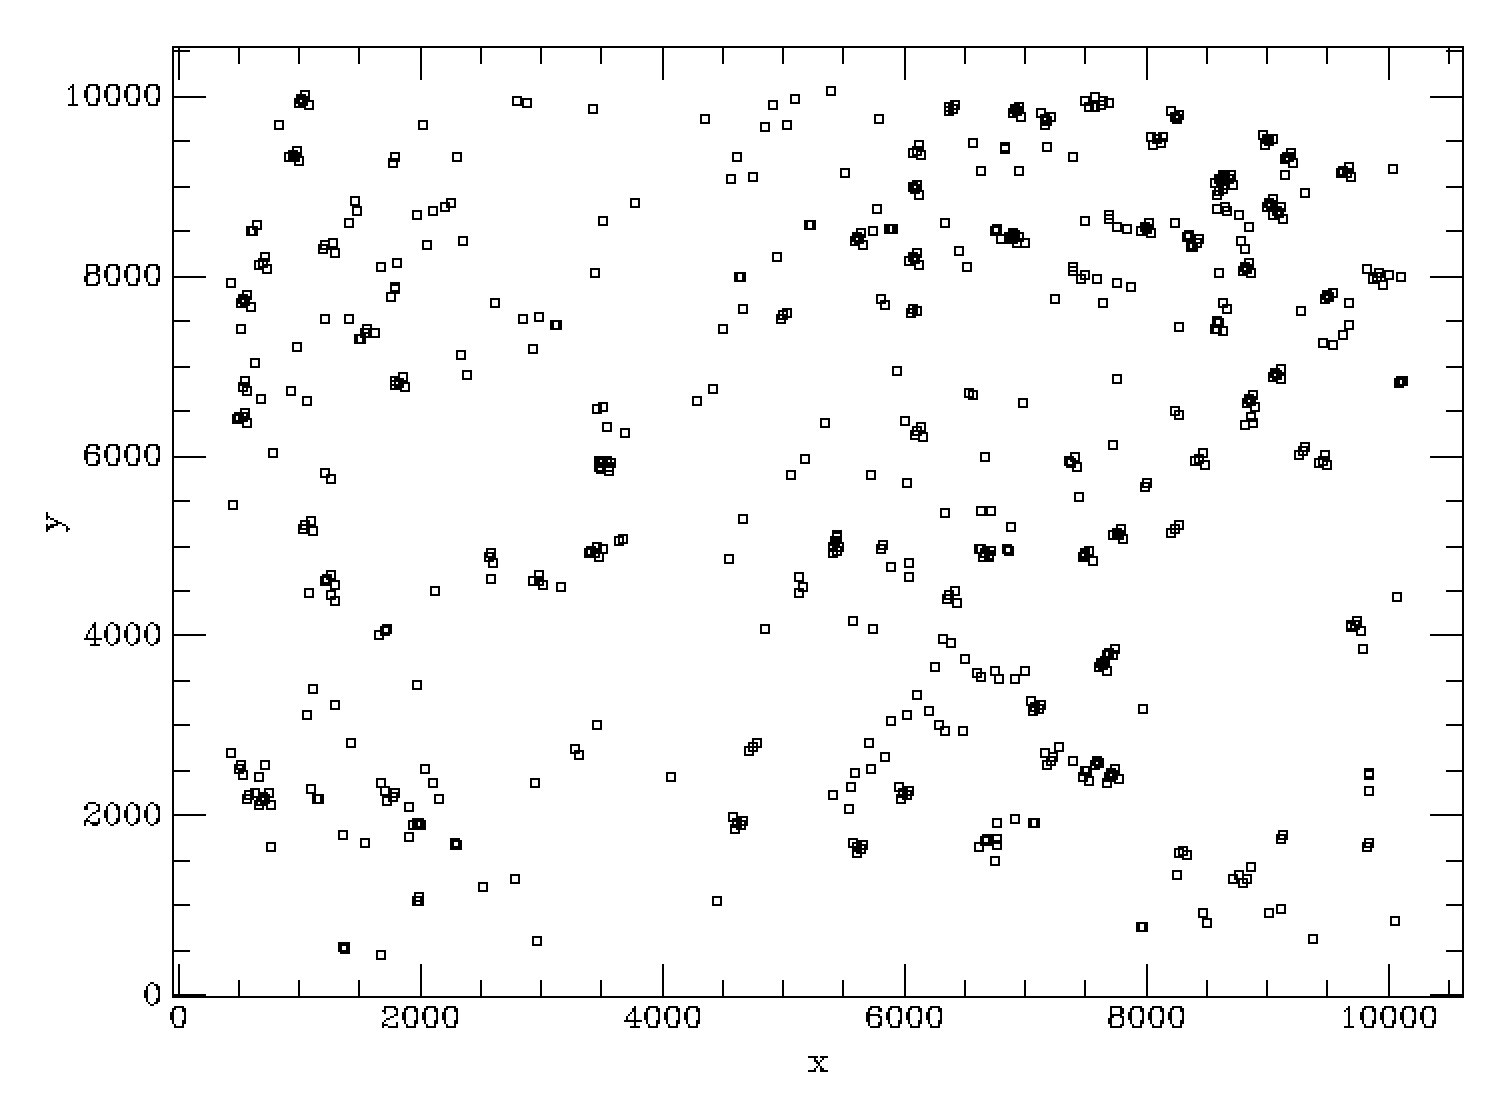
\includegraphics[width=1\linewidth]{figures/plotxy_694_good_obs.png}%
     \caption{\it \small{Of the 850 expected observations, 694 were reduced properly.  Each observation's x,y--position on the detector is represented by a black square.~\label{fig:xy}}}% Shown with red squares are the 67 observations that do not have a match in the ddt files. Blue circles are no diff files
  \end{center}%
\end{figure}



\subsection{No Match}\label{sec:nomatch}
A total of 25 expected observations lack any matches with ATLAS data.  These 25 
observations correspond to 25 distinct SNe.  Since these SNe appear in other 
observations made by ATLAS, we maintain 100\% completeness.  Of these 25 SNe, 23 
were found in ATLAS observations outside the $\pm$10~day window used.  
%
The remaining two objects were identified in reduced images.  These two SN explosions 
ended before observations were made by ATLAS and were not expected to show up in the 
difference images.
% These failed matches do not fall within the $\pm$10~day window used, due to poor observation conditions.  
%These 25 unmatched observations do not reduce our completeness, since these SNe 
%appear in other observations made by ATLAS. 



\subsection{No diff File}
\indent Missing difference images account for 49 of the expected 850 observations. 
Matches that were missing difference images can be attributed to an error in the 
ATLAS pipeline. An error during differencing caused a break in the pipeline and no 
further images were generated for that night. Such an error will be corrected once 
the data is re--reduced.


\subsection{No ddt File}
\indent For matches that were completely missing a ddt file, ddt files were missing 
for the entire night. This accounts for 15 failed matches and will be corrected by 
the next round of differencing.


\subsection{No ddt Match}\label{sec:noddtline}

\indent Of the total 850 expected matches, 67 do not show up in existing ddt files.  
Nature constantly plays a role in collecting astronomical data. When 
observations are made at the beginning or end of a night, ambient light 
levels rise and sky background fluctuations. 3 of the 67 missing ddt 
lines can be attributed to poor observation conditions, brought on by 
clouds and increased levels of sky background.\\
%
\indent Errors during the image differencing process led to the loss of 8 
expected overlaps. Older differencing techniques caused entire portions 
of images to be lost, accounting for 3 failed matches.\\
%
\indent There were 6 cases where bright host galaxies caused the SNe to become extremely 
faint in the difference image. Outdated differencing procedures lead to less 
uniform backgrounds, making it harder to identify faint objects.  
%While preforming photometric calculations, the ATLAS pipeline failed to trigger 
During photometric calculations, the ATLAS pipeline failed to trigger 
on these 6 faint objects.\\
%
\indent There are various reason why the PSF across an image may vary.  
Here, the major contributors are high levels of sky background and optical 
issues inherent to the ATLAS system.  
If not properly corrected, such issues cause observed objects to become distorted.  
Distortion can cause sharp edges to become fuzzy, resulting in the ATLAS pipeline 
failing to trigger on such objects. This accounts for 3 of the missing matches.  
Objects that were only in reduced images, but not in differenced images, account 
for 26 of the matches missing from the ddt files. Such instances arise when the 
object is fully subtracted during differencing, due to it existing in the wallpaper.  
As the wallpaper is an ongoing project, corrected future versions will not cause this issue.\\
%
\indent There were 17 cases in which the SNe was not detecting in either the reduced or 
differenced image, indicating poor astrometry. Another possible explanation is 
bad photometry. If photometry is the issue, the SN explosions must have occurred 
outside the nominal $\pm$10~day window.\\
%
\indent No two detectors are identical, since each one is handcrafted.  
As excess silicon is removed from the 
edges of a detector, minor defects are introduced.  Many of 
these defects are removed during image processing.  Corrections 
cannot be made for data that fall on the edges of a detector, 
where the silicon has been trimmed away.  To account for this, 
ATLAS observation patterns are dithered.  
This dither allows for objects that fall on the edges of the 
detector to be observed more than 5 times a night.  
The final group of matches that are missing from the ddt files 
are of objects that fall on the edges of an observation.  
Such objects only exist in one of the two overlapping observations.

\begin{figure}[h!]%[H]
\begin{center}
    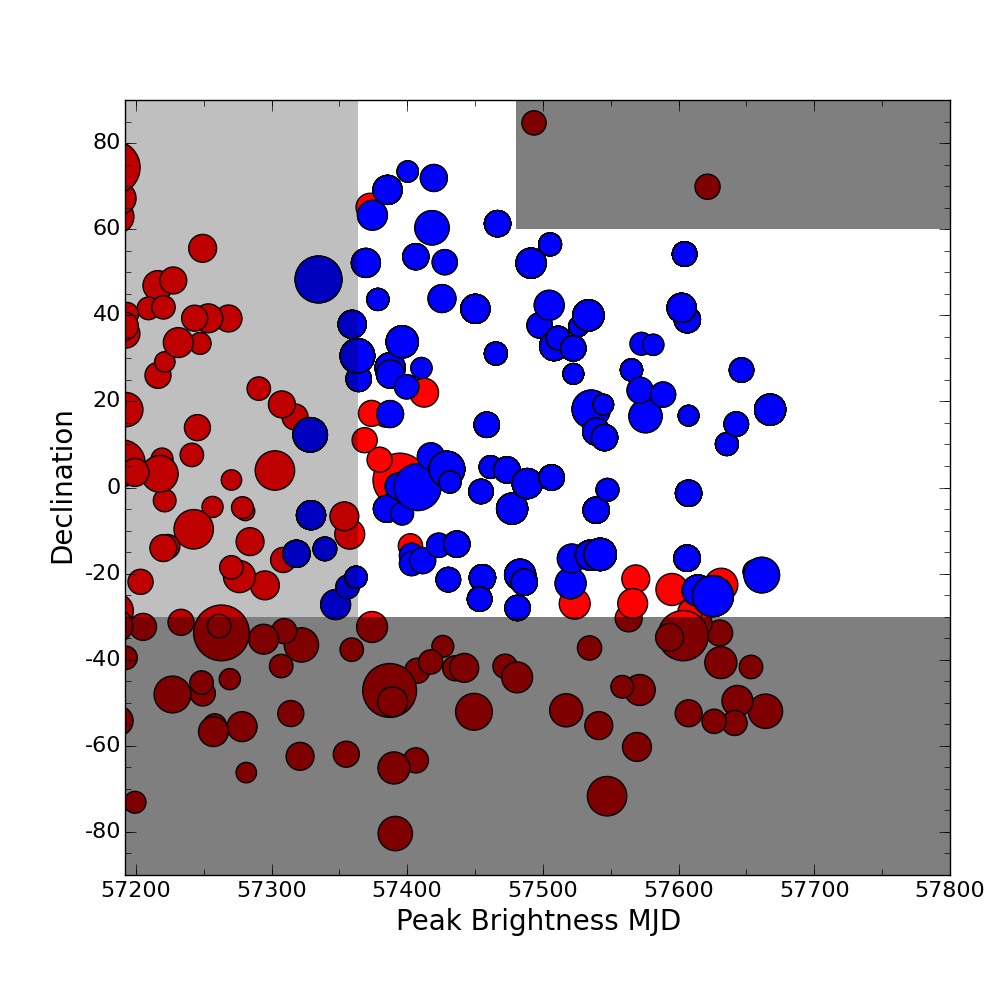
\includegraphics[width=1\linewidth]{figures/plot2useinPaper_restrictxfurther.png}%
     \caption{\it \small{ASASSN SNe that do not have matches in ATLAS data are shown in red.  SNe that were found in ATLAS observations are shown in blue.  Regions that have a lower chance of containing SNe have been covered in gray.  The lower dark gray region eliminates objects below the ATLAS observation limit of $-30\deg$.  A dark gray region starting at 57480 has been added to show when ATLAS went from 4 to 5 observations a night, giving an effective limit of Dec=$+60\deg$.  This figure has been restricted to only includes SNe discovered by ASASSN during the time ATLAS was collecting data.  The light gray region extends from ATLAS first night of collecting data up until 57364, when the reduction method was refined enough to produce usable data.~\label{fig:dec_mjd}}}
  \end{center}
\end{figure}
